%!TEX root = main.tex
\section{Backup Slides}

\begin{frame}
\frametitle{What about Gesture Detection?}

\begin{figure}[!htb]
\centering
\resizebox{\columnwidth}{!}{
	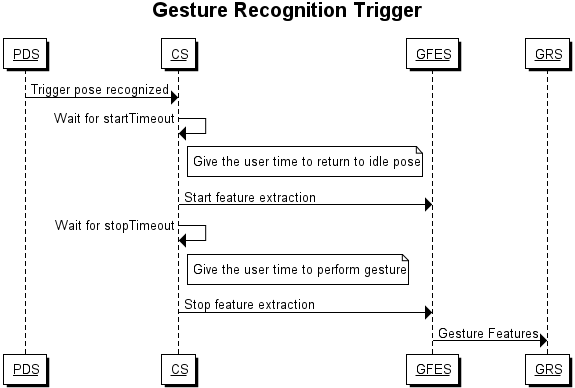
\includegraphics[]{figs/gesturerec-trigger}
}
\end{figure}

\end{frame}

\begin{frame}
\frametitle{Why not a stream of poses?}

$2$ main approaches

\begin{itemize}
\item \textbf{FSM} of intermediate poses: Every new gesture needs to be hard coded
\item \textbf{HMM} with intermediate poses as observations: Generalizes but couples recognition accuracy with frame rate / network stability
\end{itemize}

\end{frame}

\begin{frame}
\frametitle{Kinect on Raspberry Pi}

\textbf{APPROACH}

Use Windows 10 IOT Edition

\textbf{PROBLEMS}

\begin{itemize}
\item Does not support Kinect drivers and Kinect SDK
\item Not enough voltage provided through USB hub to sustain the Kinect sensor
\end{itemize}

\end{frame}



\begin{frame}
\frametitle{Kinect on Raspberry Pi}

\textbf{APPROACH}

\begin{itemize}
\item Use USB over IP to stream the low level Kinect data from a Raspberry Pi 
to a Windows Server so that it appears the Kinect sensor is connected to the server
\item Cross-Compile the Linux kernel with USB-IP modules support
\end{itemize}

\textbf{PROBLEMS}

\begin{itemize}
\item USB-IP modules do not support USB hubs
\item Bandwidth limitations
\end{itemize}

\Wider[5em] {
\begin{figure}[!htb]
\centering
\resizebox{\columnwidth}{!}{
	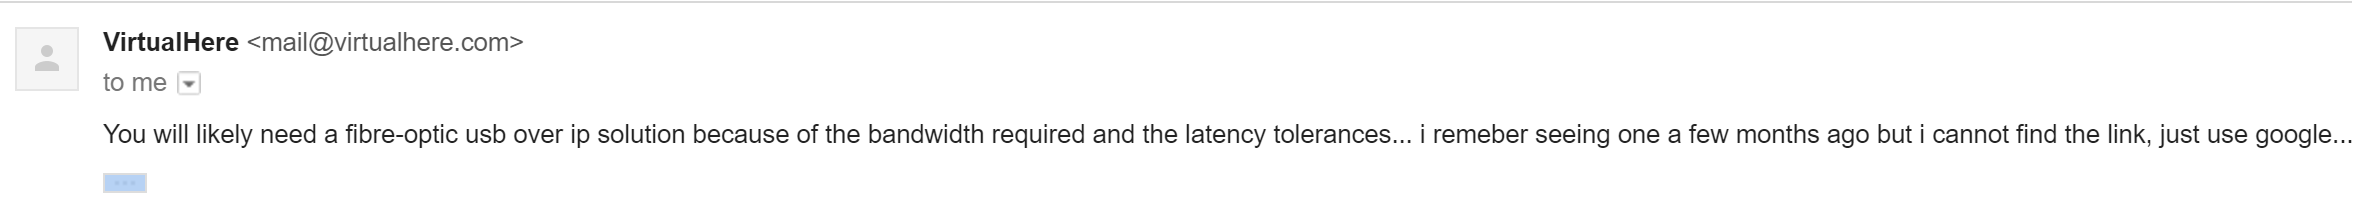
\includegraphics[]{figs/virtualhere-email}
}
\end{figure}
}
\end{frame}

\begin{frame}[fragile]
\frametitle{Why C\#? Why Python? Why JS?}

\textbf{C\#}

\begin{itemize}
\item \texttt{Kinect SDK}
\end{itemize}

\textbf{Python}

\begin{itemize}
\item \texttt{scikit-learn}
\end{itemize}

\textbf{JS}
\begin{itemize}
\item 
\begin{lstlisting}[
    basicstyle=\footnotesize, %or \small or \footnotesize etc.
]
  async.parallel(
    // List of pose detectors to run concurrently
    Object.keys(poseDetectors)
      .reduce((prev, pose) => {
        prev[pose] = poseDetectors[pose](features)
        return prev
      }, {}),
    (err, result) => {
      /* handle list of results ... */
    })
\end{lstlisting}

\end{itemize}

\end{frame}

